\chapter{Modelul de inteligență artificială și setul de date}

Componenta de analiză media din WhereWeFishin se bazează pe un model de detecție de obiecte antrenat pe un set de date creat și adnotat manual. Acest capitol detaliază procesul complet: de la colectarea imaginilor și adnotarea lor, prin antrenarea și evaluarea modelului, până la integrarea sa în serviciul Python de producție. Această componentă reprezintă contribuția cea mai distinctivă a proiectului față de o aplicație web convențională de rezervări.

\section{Contextul și motivația unui set de date dedicat}

Modelele YOLO preantrenate pe seturi de date publice de referință (precum COCO \citep{lin2014coco}) nu conțin o clasă dedicată peștilor. Setul COCO, cu cele 80 de categorii ale sale, nu include pești, ceea ce face imposibilă folosirea directă a unui model generic pentru identificarea capturilor. Această absență a justificat construirea unui set de date propriu: fără el, platforma nu ar putea oferi nicio informație despre specia peștelui fotografiat sau filmat.

Alternativele disponibile public, seturi de date de pești pentru medii marine sau subacvatice controlate, au o distribuție a speciilor diferită față de realitatea pescuitului recreativ din România. Specii comune în apele locale, precum crapul, ctenoul, șalăul sau știuca, sunt subreprezentate sau absente în aceste seturi. Din acest motiv, crearea unui set de date propriu, adaptat contextului local și condițiilor reale de captare a imaginilor, a fost o alegere necesară, nu opțională.

\section{Colectarea și structura setului de date}

Imaginile au fost colectate din surse variate: fotografii proprii realizate în condiții de pescuit recreativ, capturi de ecran extrase din videoclipuri de pescuit și imagini adnotabile disponibile public. Diversitatea surselor este importantă pentru a evita supraspecializarea modelului pe un singur tip de iluminare, unghi sau fundal.

Setul de date include mai multe clase de specii de pești frecvent întâlnite în contextul pescuitului recreativ, fiecare reprezentată prin imagini cu variații de poziție, unghi de vizualizare, distanță față de cameră și condiții de lumină. Clasele acoperă atât pești capturați și fotografiați în afara apei, cât și exemplare vizibile la suprafața apei sau în condiții de vizibilitate parțială.

Structura finală a setului de date urmează convenția Ultralytics YOLO: directoarele \texttt{train}, \texttt{val} și \texttt{test} conțin imagini și etichete asociate. Fiecare imagine are un fișier de etichete cu același nume, în format text, unde fiecare linie descrie un obiect prin indexul clasei și coordonatele bounding box-ului normalizate.

Figura~\ref{fig:dataset-stats} prezintă o analiză cantitativă a setului de date generată automat de pipeline-ul Ultralytics: distribuția numărului de instanțe pe clasă, suprapunerea bounding box-urilor centrate în origine și distribuțiile 2D ale poziției centrelor (\textit{x}, \textit{y}) și dimensiunilor (\textit{width}, \textit{height}) pe imaginile setului de antrenare. Aceste reprezentări sunt utile pentru detectarea dezechilibrelor: clasele cu sub 600 de instanțe (precum \emph{MorishIdol} sau \emph{RibbonedSweetlips}) sunt subreprezentate și vor avea probabil performanță mai scăzută. Distribuția dimensiunilor arată o concentrare a obiectelor mici și medii, iar distribuția pozițiilor este centrată, ceea ce reflectă tendința naturală a fotografiilor de a centra subiectul principal.

\begin{figure}[H]
\centering
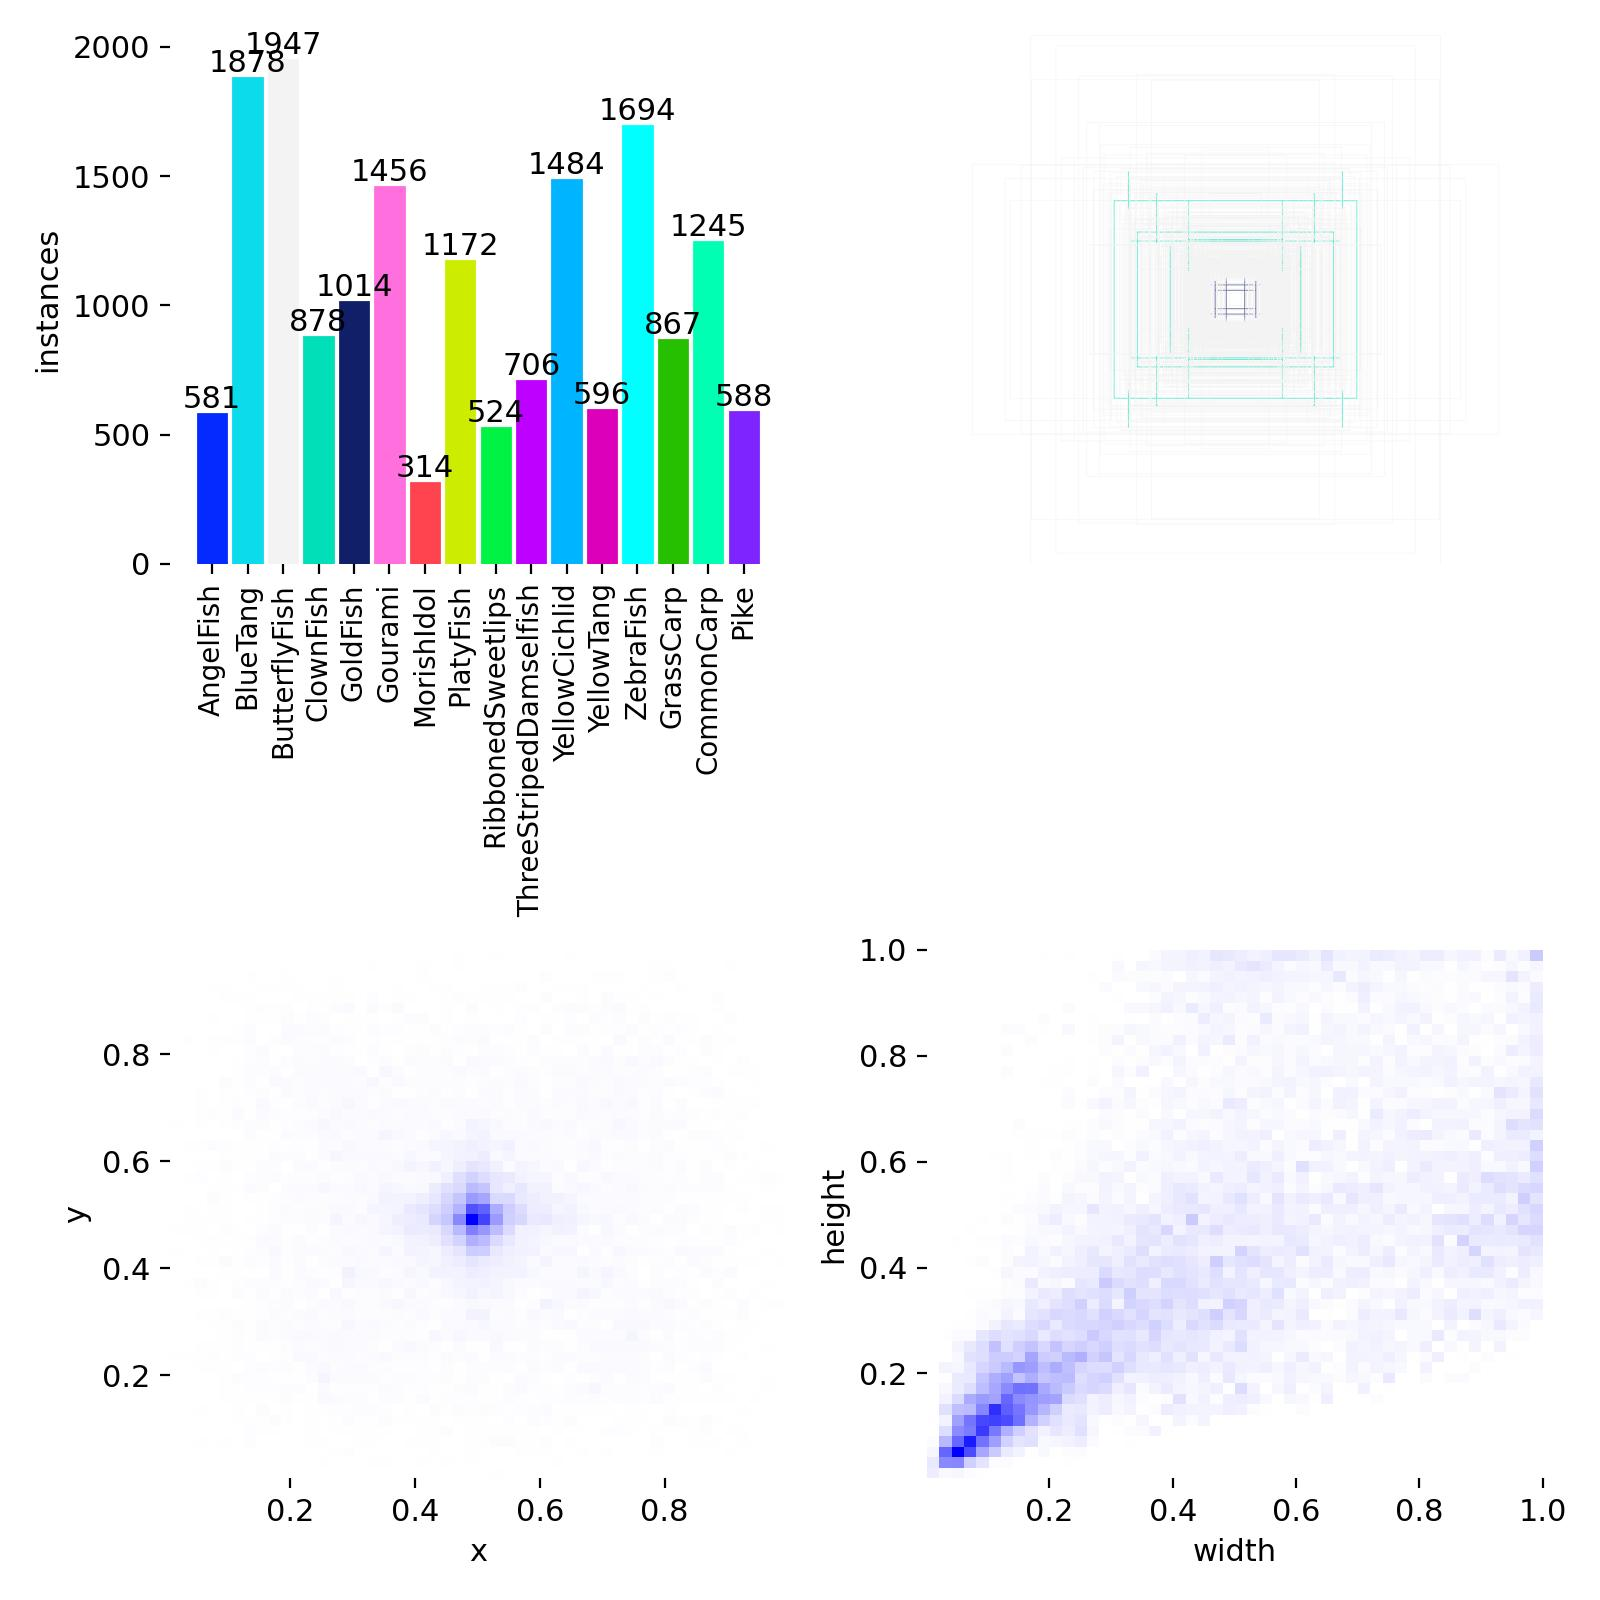
\includegraphics[width=\textwidth]{images/labels.jpg}
\caption{Statistici ale setului de date: distribuția numărului de instanțe pe clasă, suprapunerea bounding box-urilor și distribuțiile 2D ale pozițiilor și dimensiunilor obiectelor}
\label{fig:dataset-stats}
\end{figure}

\needspace{10\baselineskip}
\begin{lstlisting}[language=bash, caption={Exemplu de fișier de adnotare YOLO pentru o imagine cu doi crapi și o stiuca}]
# <clasa>  <cx>    <cy>    <w>     <h>
0           0.512   0.438   0.324   0.671
0           0.231   0.689   0.198   0.412
1           0.764   0.312   0.155   0.283
\end{lstlisting}

Fiecare linie corespunde unui pește detectat în imagine. Indexul clasei (\texttt{0} = crap, \texttt{1} = stiuca) este urmat de coordonatele centrului bounding box-ului (\texttt{cx}, \texttt{cy}) și de lățimea și înălțimea acestuia (\texttt{w}, \texttt{h}), toate normalizate în intervalul \([0, 1]\) față de dimensiunile imaginii. Această structură este consumată direct de pipeline-ul de antrenare fără preprocesare suplimentară.

\section{Adnotarea și preprocesarea imaginilor}

Adnotarea bounding box-urilor a fost realizată manual pentru fiecare imagine din setul de date. Instrumentul de adnotare utilizat permite marcarea vizuală a zonelor de interes și exportul direct în formatul YOLO, eliminând conversia manuală a coordonatelor. Adnotarea a urmărit principiul delimitării stricte a corpului peștelui, excluzând umbra sau reflecția apei, pentru a reduce zgomotul din semnalul de antrenare.

Preprocesarea și augmentarea datelor au fost aplicate în cadrul pipeline-ului de antrenare. Augmentările includ oglindire orizontală, rotații ușoare, ajustări de luminozitate și contrast, zoom aleatoriu și mozaic, adică combinarea a patru imagini într-una singură, o tehnică specifică familiei YOLO care îmbunătățește detecția obiectelor la scări variate. Aceste transformări măresc artificial diversitatea setului de antrenare și reduc riscul de overfitting la condițiile specifice imaginilor originale.

\section{Antrenarea modelului}

Modelul utilizat face parte din familia YOLOv8, implementată prin biblioteca Ultralytics \citep{ultralytics}. Alegerea acestei versiuni este justificată de echilibrul dintre acuratețe și viteză de predicție, de suportul nativ pentru antrenare pe GPU și de integrarea facilă cu PyTorch \citep{pytorch}. Familia YOLOv8 menține arhitectura unui singur pas, de tip \emph{single-stage detector}, care estimează simultan localizarea și clasificarea, ceea ce o face potrivită atât pentru imagini, cât și pentru analiza video cadru cu cadru \citep{redmon2016yolo}.

Antrenarea a pornit de la greutăți preantrenate pe setul COCO \citep{lin2014coco}, folosind tehnica de transfer learning \citep{goodfellow2016,bishop2006}. Rețeaua a preluat reprezentările generale de viziune din antrenarea inițială și a rafinat straturile finale pe setul de date propriu, adăugând clasele de specii de pești absente din setul original. Această abordare reduce semnificativ numărul de epoci necesare pentru convergență și îmbunătățește stabilitatea antrenamentului față de inițializarea de la zero.

Configurația de antrenare a inclus un număr de epoci ales în funcție de curbele de convergență observate, cu monitorizarea continuă a training loss-ului și a metricilor de validare. S-a utilizat un mecanism de early stopping pentru a preveni overfitting-ul: antrenamentul se oprește automat dacă metrica principală nu se îmbunătățește pe un număr definit de epoci consecutive. Dimensiunea batch-ului a fost adaptată la memoria GPU disponibilă, iar learning rate-ul a urmat un scheduler cu descreștere lentă pe parcursul antrenamentului.

Figura~\ref{fig:curbe-antrenare} prezintă curbele de evoluție pentru cele 100 de epoci ale antrenamentului final. Pe rândul superior sunt afișate cele trei componente ale training loss-ului (\textit{box\_loss}, \textit{cls\_loss}, \textit{dfl\_loss}) și metricile de precizie și recall calculate pe setul de validare la fiecare epocă. Toate cele trei loss-uri prezintă o descreștere monotonă, cu o scădere accentuată în primele 10--20 de epoci urmată de o convergență lentă. Rândul inferior afișează aceleași loss-uri calculate pe setul de validare, împreună cu metricile mAP@0.5 și mAP@0.5--0.95. Convergența este stabilă, fără semne de overfitting: loss-urile de validare se stabilizează la valori comparabile cu cele de antrenare, iar metricile mAP cresc consistent până la atingerea unui platou. Spike-urile inițiale din loss-urile de validare reflectă instabilitatea normală a primelor epoci de transfer learning, în care straturile finale ale rețelei sunt rapid recalibrate pe noul set de clase.

\begin{figure}[H]
\centering
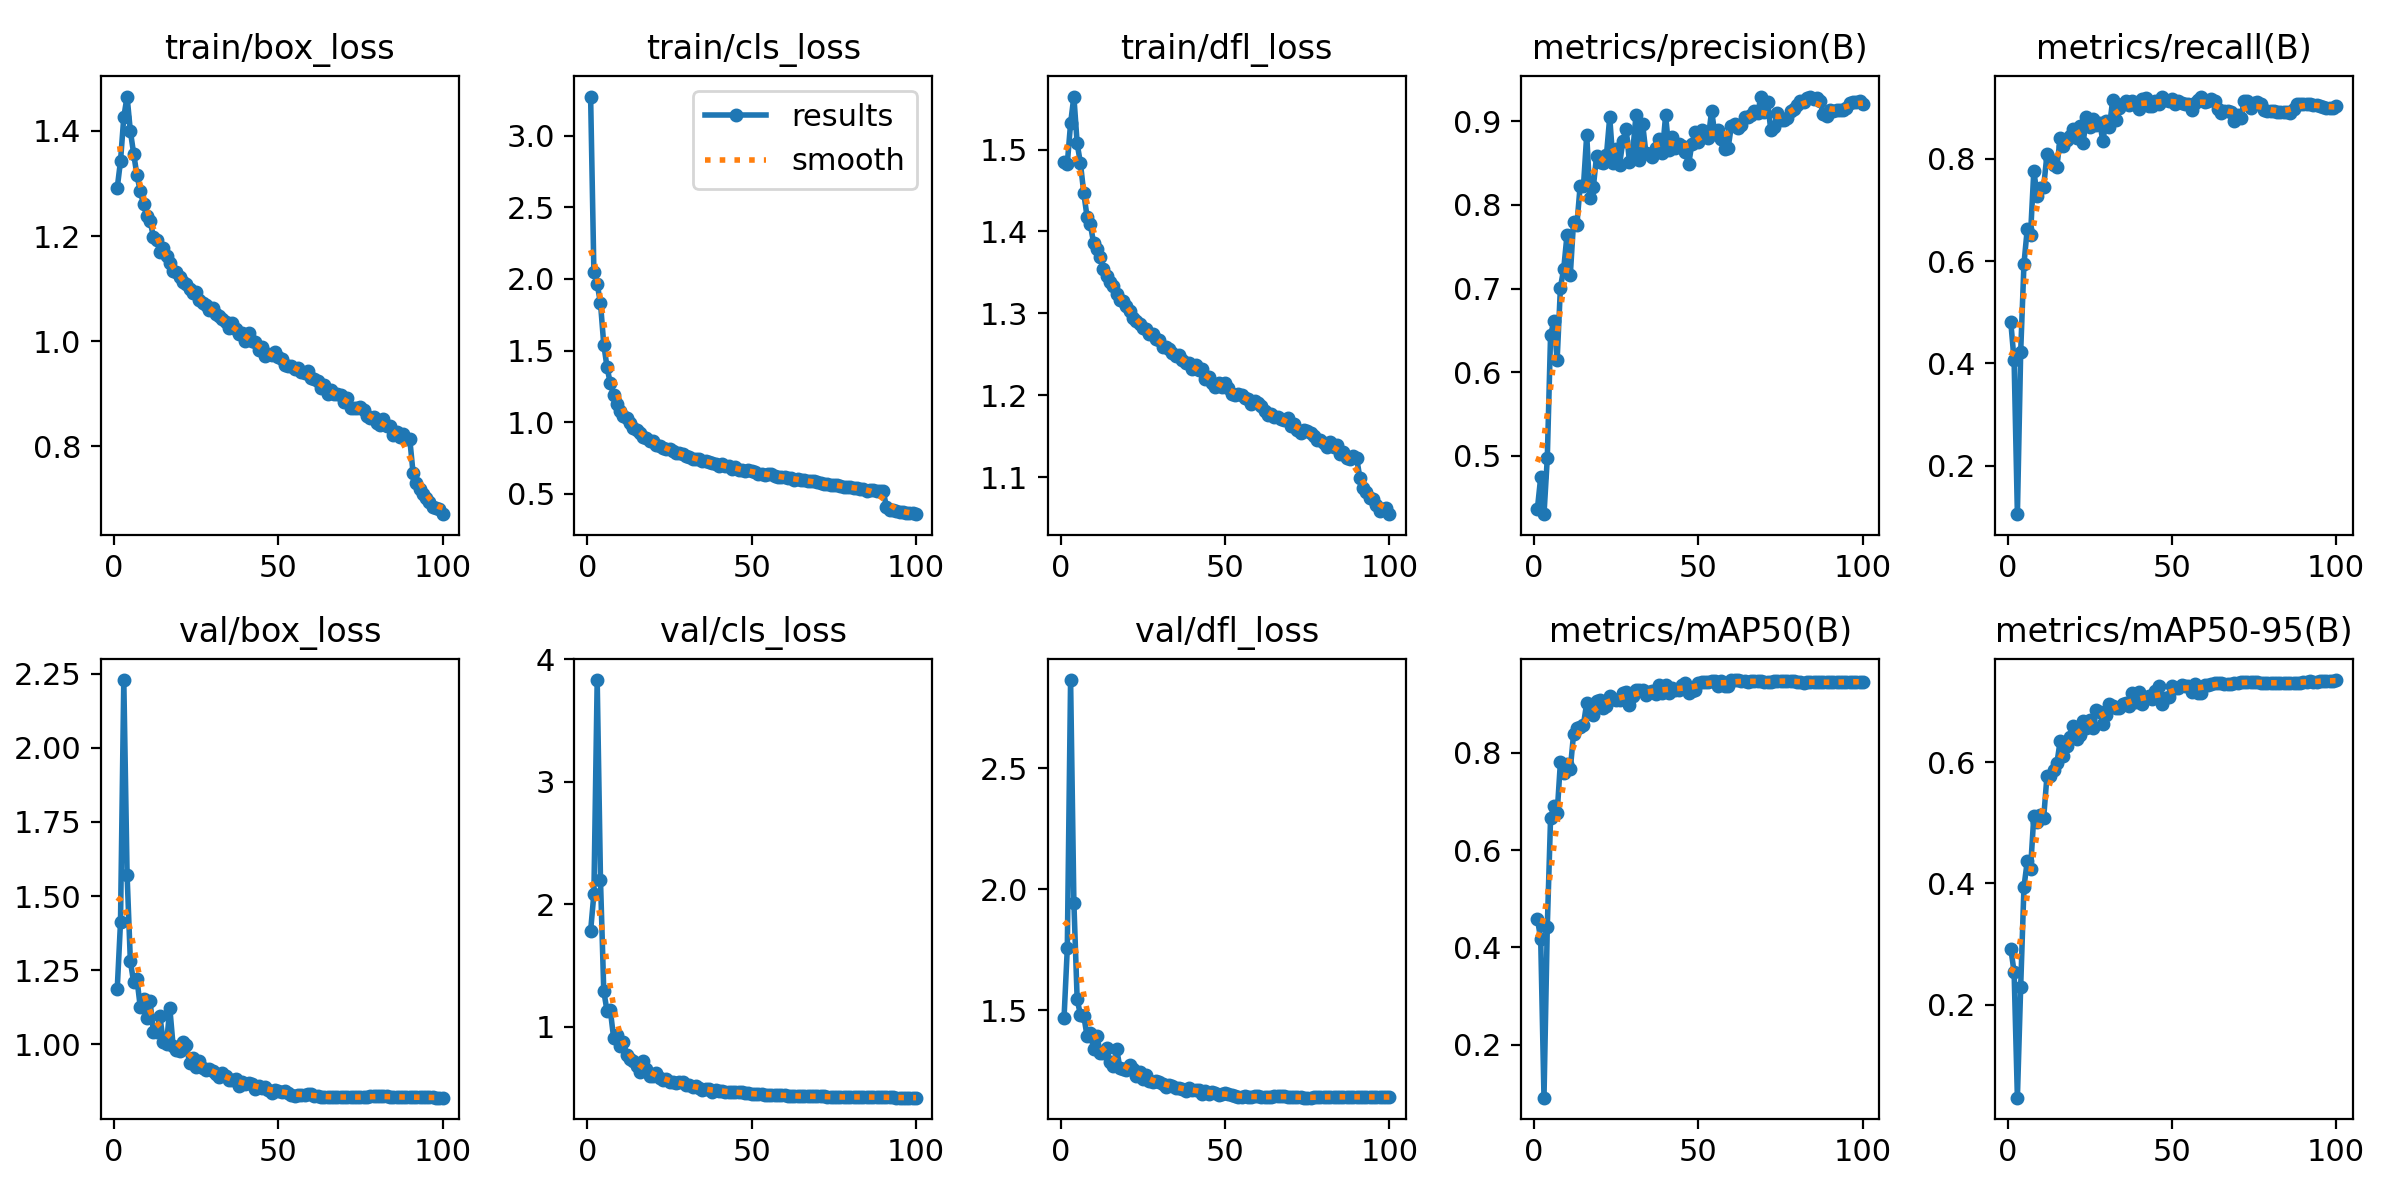
\includegraphics[width=\textwidth]{images/results.png}
\caption{Curbele de antrenare YOLOv8 pe 100 de epoci: loss-uri (box, cls, dfl) și metrici (precision, recall, mAP@0.5, mAP@0.5--0.95) pentru seturile de antrenare și validare}
\label{fig:curbe-antrenare}
\end{figure}

\section{Evaluarea performanței modelului}

Evaluarea modelului s-a realizat pe setul de test rezervat, care nu a participat la antrenare sau la selecția hiperparametrilor. Metricile principale utilizate sunt cele standard pentru detecția de obiecte: precizia (P), recall-ul (R) și media preciziei medii la un prag de IoU de 0.5 (mAP@0.5).

Precizia (P) măsoară câte dintre detecțiile returnate de model sunt corecte, raportând detecțiile adevărat pozitive la suma dintre adevărat pozitive și fals pozitive. Recall-ul (R) măsoară câte dintre obiectele reale au fost detectate, raportând adevărat pozitivele la suma dintre adevărat pozitive și fals negative. Valoarea F1, media armonică dintre precizie și recall, oferă o metrică unificată utilă mai ales când distribuția claselor este dezechilibrată.

Pragul de IoU (Intersection over Union) de 0.5 reprezintă criteriul standard de acceptare: o detecție este considerată corectă dacă bounding box-ul prognozat se suprapune cu cel de referință în proporție de cel puțin 50\%. Metrica mAP@0.5--0.95 extinde acest criteriu calculând media mAP la praguri mai stricte (până la 0.95 cu pas de 0.05), penalizând mai puternic localizările imprecise chiar dacă clasificarea speciei este corectă.

Figura~\ref{fig:metrici-model} sintetizează relația dintre principalele metrici de evaluare utilizate în analiza performanței modelului.

\begin{figure}[H]
\centering
\begin{tikzpicture}[
  every node/.style={font=\small},
  met/.style={draw, rounded corners, align=center, minimum width=4.5cm, minimum height=1.3cm, fill=gray!10, line width=0.7pt},
  arrow/.style={-Latex, thick}
]
\node[met] (prec) at (0, 0)     {Precizie (P)};
\node[met] (rec)  at (9, 0)     {Recall (R)};
\node[met] (map)  at (4.5, -3.0){mAP@0.5};
\node[met] (f1)   at (4.5, -6.0){F1 Score};
\draw[arrow] (prec) -- node[font=\footnotesize, fill=white, inner sep=2pt]{contribuie la} (map);
\draw[arrow] (rec)  -- node[font=\footnotesize, fill=white, inner sep=2pt]{contribuie la} (map);
\draw[arrow] (prec) to[bend right=12] node[font=\footnotesize, fill=white, inner sep=2pt, left]{combinate} (f1);
\draw[arrow] (rec)  to[bend left=12]  node[font=\footnotesize, fill=white, inner sep=2pt, right]{în} (f1);
\end{tikzpicture}
\caption{Relația dintre metricile principale de evaluare a modelului}
\label{fig:metrici-model}
\end{figure}

\begin{figure}[H]
\centering
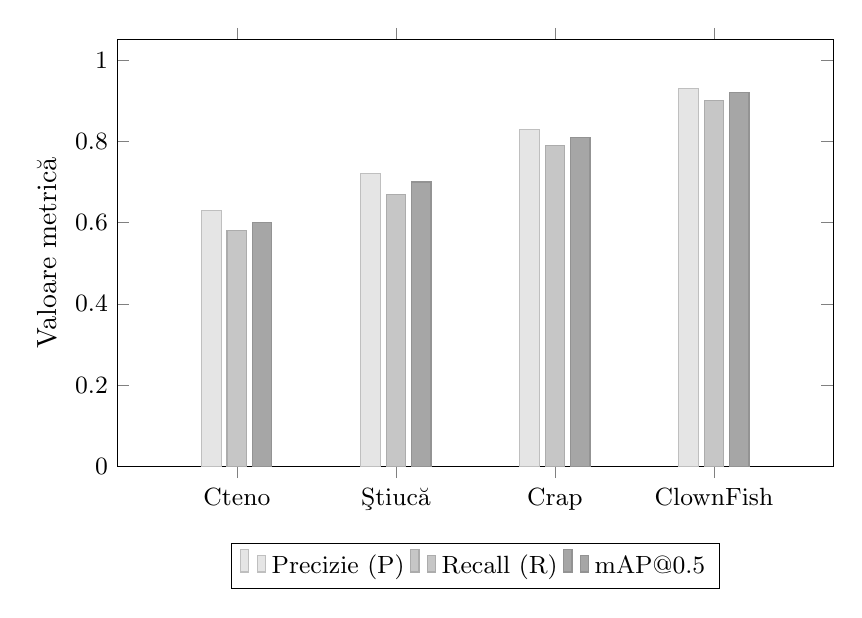
\begin{tikzpicture}
\begin{axis}[
  ybar,
  bar width=0.25cm,
  width=0.88\textwidth,
  height=7cm,
  ylabel={Valoare metrică},
  xtick={1,2,3,4},
  xticklabels={Cteno, \c{S}tiucă, Crap, ClownFish},
  x tick label style={font=\small},
  y tick label style={font=\small},
  ymin=0, ymax=1.05,
  ytick={0,0.2,0.4,0.6,0.8,1.0},
  legend style={at={(0.5,-0.18)}, anchor=north, legend columns=3, font=\small},
  legend entries={Precizie (P), Recall (R), mAP@0.5},
  enlarge x limits=0.25,
]
\addplot[fill=gray!20, draw=gray!50] coordinates {(1,.63)(2,.72)(3,.83)(4,.93)};
\addplot[fill=gray!45, draw=gray!65] coordinates {(1,.58)(2,.67)(3,.79)(4,.90)};
\addplot[fill=gray!70, draw=gray!85] coordinates {(1,.60)(2,.70)(3,.81)(4,.92)};
\end{axis}
\end{tikzpicture}
\caption{Precizie, Recall și mAP@0.5 per clasă pe setul de test}
\label{fig:metrici-per-clasa}
\end{figure}

Precizia măsoară proporția detecțiilor corecte din totalul detecțiilor efectuate, indicând câte dintre predicțiile modelului sunt reale. Recall-ul măsoară proporția obiectelor reale detectate corect, indicând câți pești au fost identificați din totalul celor prezenți în imagini. mAP@0.5 agregă aceste metrici pe toate clasele și la pragul de IoU de 0.5, oferind o imagine globală a performanței. Aceste metrici sunt formalizate în literatura de specialitate \citep{powers2011} și reprezintă standardul \emph{de facto} pentru raportarea rezultatelor în detecția de obiecte, fiind folosite în lucrările de referință din domeniu (Pascal VOC \citep{everingham2010pascal}, COCO \citep{lin2014coco}).

Performanța variază între clase, reflectând dificultățile specifice fiecărei specii: dimensiunile tipice ale peștelui în imagine, diversitatea aspectului vizual și frecvența reprezentării în setul de antrenare. Clasele cu mai multe exemple și mai puțină variabilitate morfologică obțin metrici mai ridicate. Clasele mai rare sau cu aspect vizual similar altor specii prezintă valori mai mici, ceea ce indică direcții clare de extindere a setului de date.

Matricea de confuzie a modelului permite identificarea erorilor sistematice: confundarea speciilor cu aspect similar și detecțiile false în zone cu textură asemănătoare (suprafața apei, vegetație subacvatică). Aceste observații ghidează colectarea ulterioară de date: speciile confundate au nevoie de exemple suplimentare variate, iar imaginile cu fundal complex contribuie direct la reducerea falselor pozitive.

Figura~\ref{fig:predictii-validare} prezintă un set de predicții ale modelului pe imagini din setul de validare pentru clasa \emph{Pike} (știuca). Bounding box-urile generate de model încadrează corect peștele în diverse contexte: subacvatic cu iluminare slabă, fotografii cu pescari ținând captura, imagini de studio pe fundaluri neutre și capturi naturale pe vegetație. Această diversitate de contexte vizuale validează capacitatea modelului de a generaliza dincolo de condițiile specifice imaginilor de antrenare. Detecțiile sunt etichetate corect chiar și atunci când peștele ocupă doar o parte mică din cadru sau este parțial obstrucționat de mâna pescarului, ceea ce confirmă robustețea adusă de augmentările aplicate în timpul antrenării (oglindire, scalare, mozaic).

\begin{figure}[H]
\centering
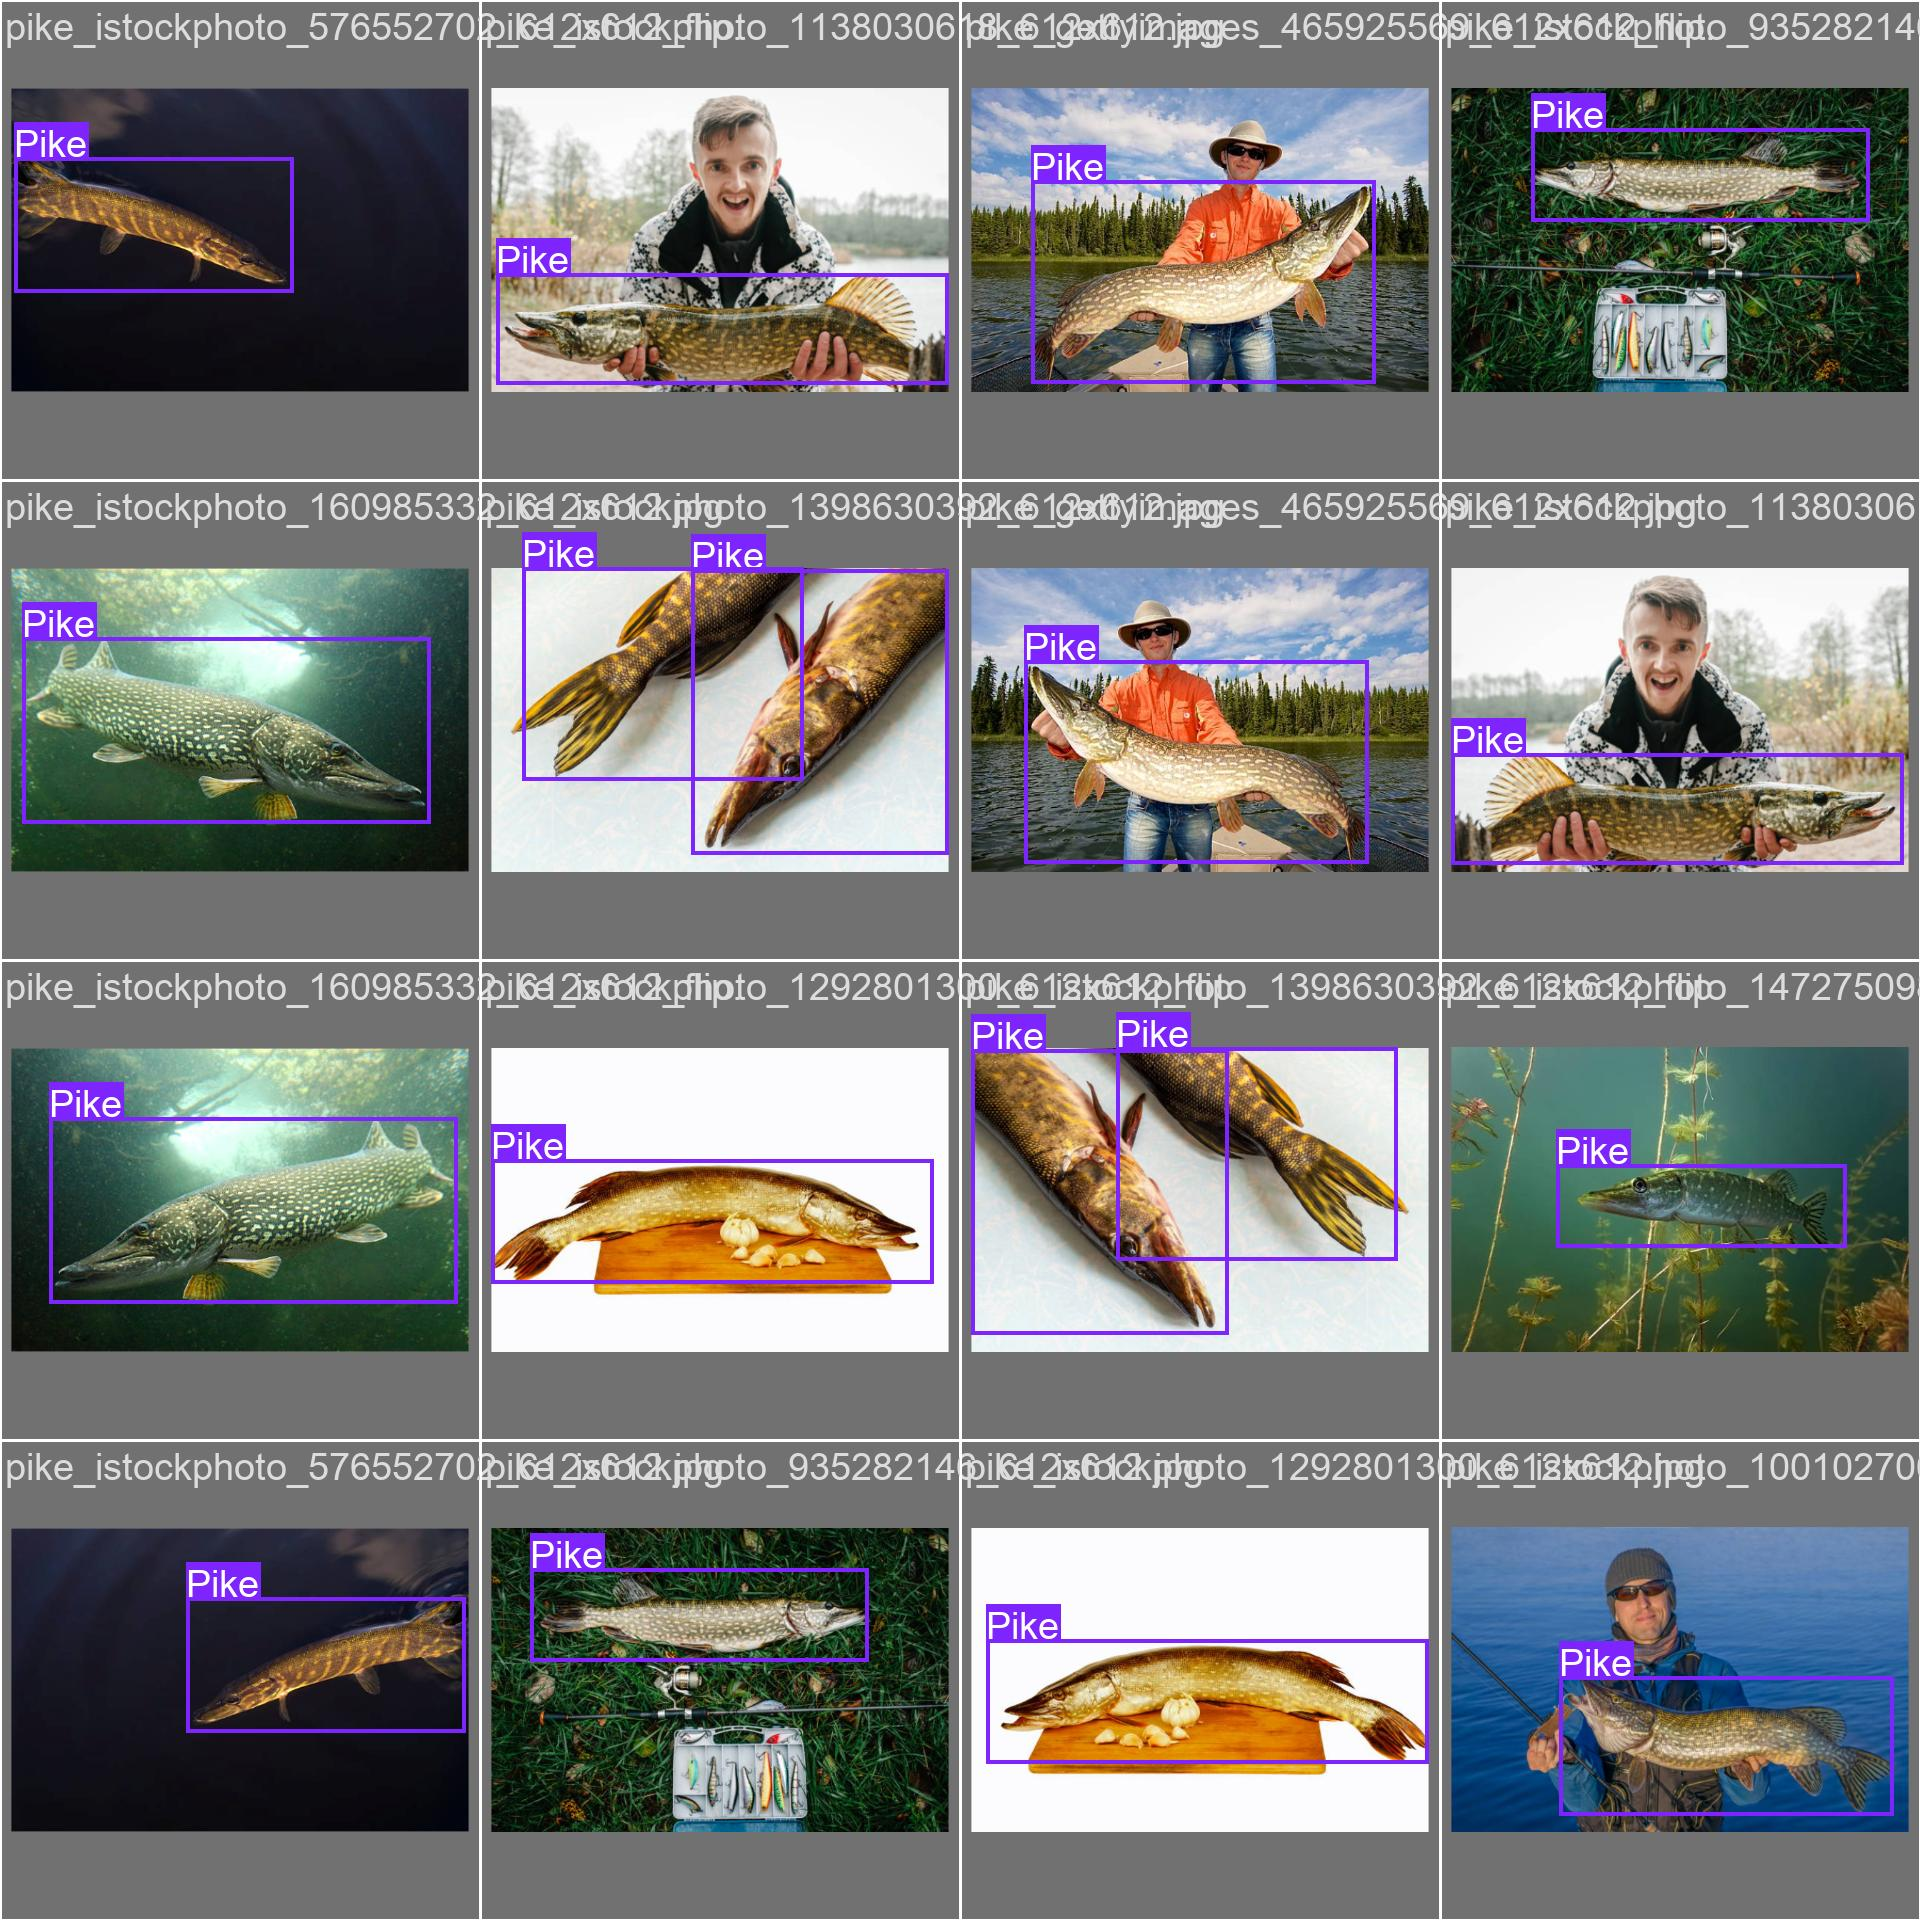
\includegraphics[width=\textwidth]{images/val_batch1_labels.jpg}
\caption{Predicții ale modelului pe setul de validare pentru clasa \emph{Pike}: bounding box-uri generate automat pe imagini cu contexte și unghiuri variate}
\label{fig:predictii-validare}
\end{figure}

\section{Integrarea modelului antrenat în producție}

Modelul antrenat este exportat în formatul \texttt{.pt} (PyTorch checkpoint) și inclus în directorul serviciului Python Flask. La pornirea serviciului, modelul este încărcat o singură dată în memorie și reutilizat pentru toate cererile de analiză, evitând overhead-ul repetitiv al inițializării.

Pragul de încredere pentru detecție este configurat explicit și a fost ales pe baza curbelor de precizie-recall observate pe setul de validare: o valoare prea mică include detecții nesigure care produc zgomot vizual, iar o valoare prea mare exclud detecții corecte cu grad de încredere moderat. Pragul ales reprezintă un compromis care favorizează precizia față de recall, deoarece în contextul aplicației o detecție incertă este mai problematică decât o detecție lipsă.

Pentru analiza video, modelul este aplicat cadru cu cadru, iar rezultatele sunt transmise tracker-ului ByteTrack \citep{zhang2022bytetrack} care menține identitatea obiectelor de-a lungul secvenței. Față de abordări anterioare precum SORT \citep{bewley2016sort}, ByteTrack păstrează și detecțiile cu grad de încredere scăzut, ceea ce reduce fragmentarea traseelor atunci când peștele este parțial acoperit sau iese temporar din cadru. Această separare clară între detecție și tracking permite înlocuirea sau actualizarea modelului de detecție fără a modifica logica de urmărire temporală și invers.

ByteTrack asociază fiecărui pește detectat un identificator unic, păstrat pe parcursul întregii secvențe video atât timp cât exemplarul rămâne vizibil. Dacă peștele iese temporar din cadru și revine, algoritmul încearcă să-l reidentifice pe baza poziției anterioare și a caracteristicilor detecției. Această persistență a identității este esențială pentru numărarea corectă a exemplarelor distincte: fără tracking, un singur pește care apare în 100 de cadre ar fi contorizat de 100 de ori, generând statistici complet eronate. Cu tracking activ, același pește contribuie cu o singură unitate la totalul speciei sale.

Suprapunerea vizuală a rezultatelor pe video se realizează prin desenarea bounding box-urilor color asociate fiecărui identificator, însoțite de eticheta speciei și gradul de încredere al detecției. Contorul cumulativ de exemplare unice este actualizat în timp real și afișat în colțul superior al fiecărui cadru procesat, oferind utilizatorului o imagine imediată a activității înregistrate.

Reîncodarea finală a videoclipului procesat utilizează FFmpeg cu codecul H.264, care oferă un echilibru bun între dimensiunea fișierului rezultat și compatibilitatea cu majoritatea browserelor și dispozitivelor. Această alegere permite redarea directă în pagina web prin elementul HTML \texttt{video}, fără conversii sau plugin-uri suplimentare la client. Figura~\ref{fig:tracking-video-frame} ilustrează un cadru extras dintr-un videoclip procesat în aceste condiții.

\begin{figure}[htbp]
\centering
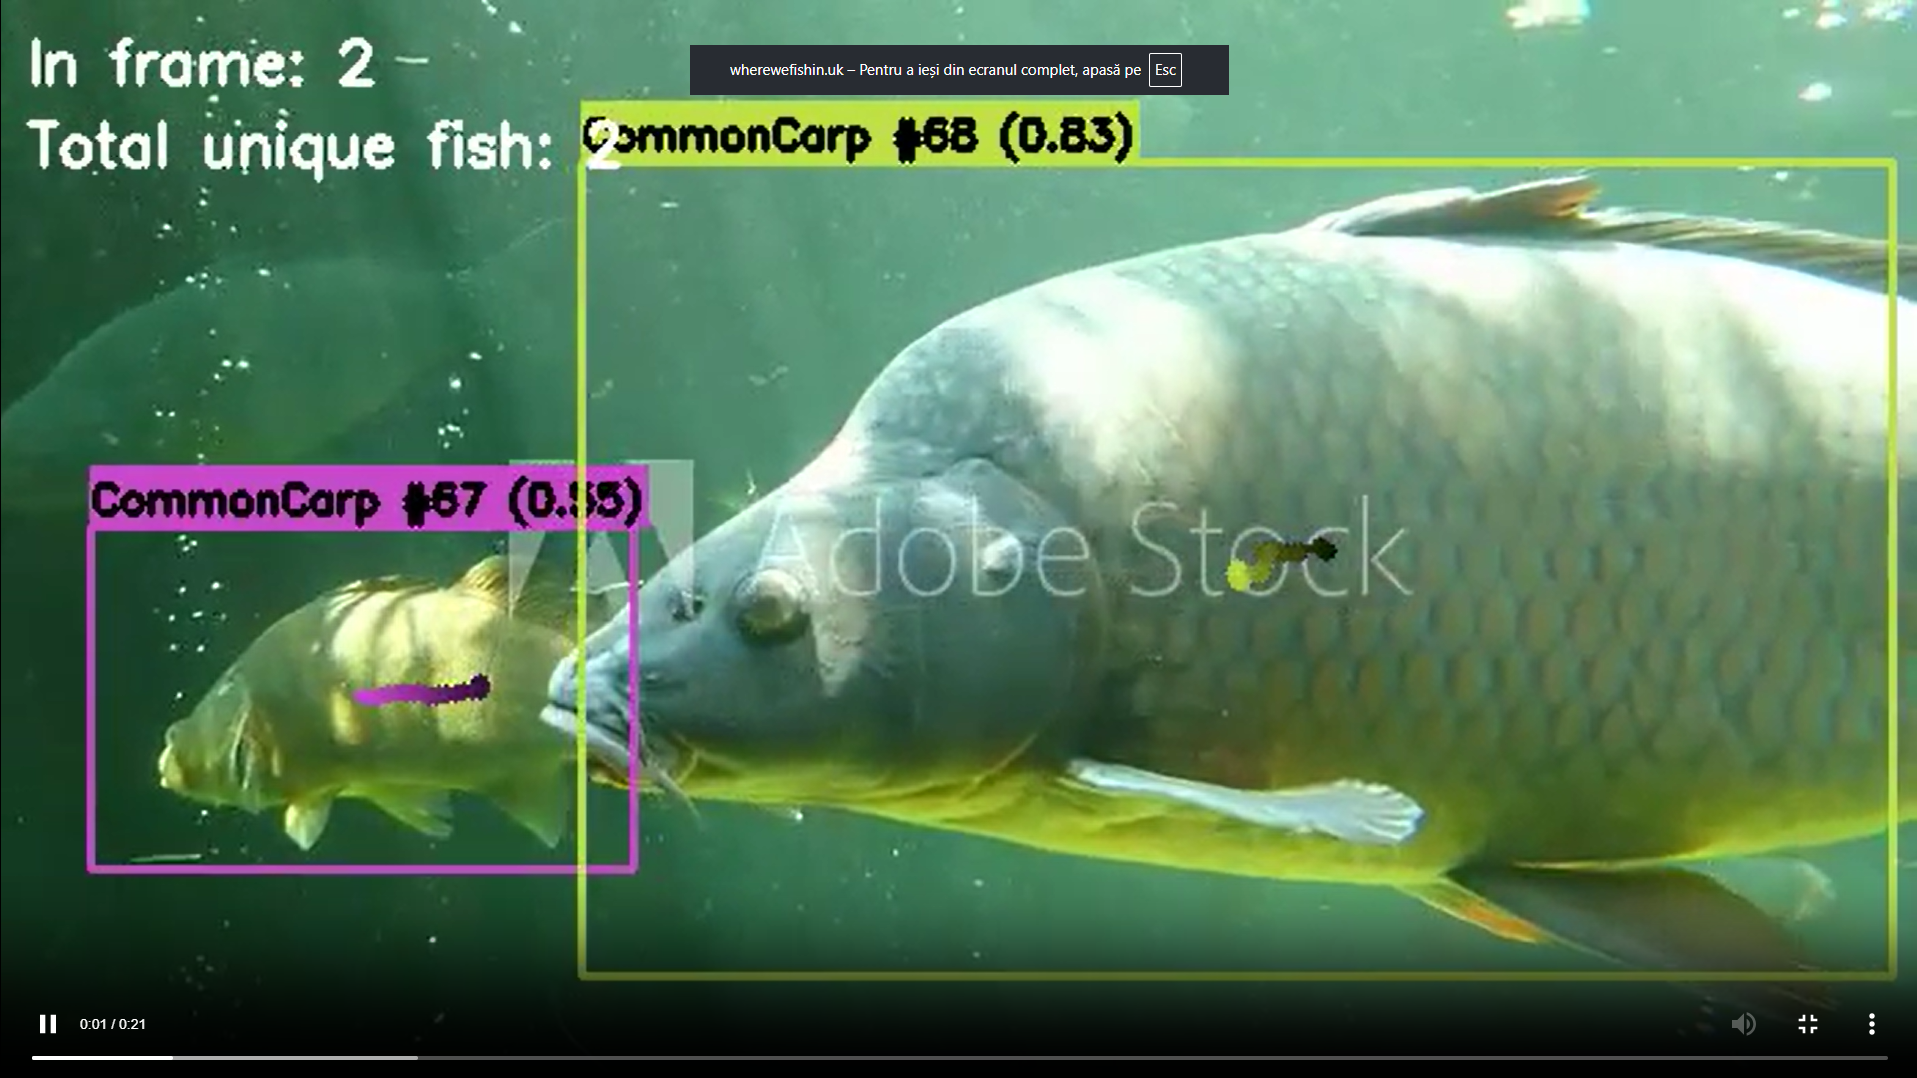
\includegraphics[width=\textwidth]{images/fish-recogResult.png}
\caption{Frame dintr-un videoclip procesat: detecție YOLOv8 cu bounding box-uri și ID-uri de tracking ByteTrack}
\label{fig:tracking-video-frame}
\end{figure}

Serviciul expune un endpoint de predicție care primește un fișier media, determină tipul de analiză (imagine sau video) pe baza tipului MIME și returnează un răspuns structurat cu detecțiile, statisticile și, în cazul video, un fișier reîncodat cu adnotările suprapuse.

\begin{lstlisting}[language=Python, caption={Endpoint Flask pentru rularea modelului YOLO}]
model = YOLO("model.pt")  # incarcat o singura data la pornire

@app.route("/analyze", methods=["POST"])
def analyze():
    if "file" not in request.files:
        return jsonify({"error": "No file provided"}), 400

    file  = request.files["file"]
    mime  = file.content_type

    if mime.startswith("image/"):
        results = run_image_inference(file, model)
    elif mime.startswith("video/"):
        results = run_video_inference(file, model)
    else:
        return jsonify({"error": "Unsupported media type"}), 415

    return jsonify({
        "detections":      results["detections"],
        "species_summary": results["species_summary"],
        "total_count":     results["total_count"],
    })
\end{lstlisting}

\section{Limitări și observații ale modelului}

Performanța modelului este influențată de condițiile în care sunt realizate fotografiile sau videoclipurile. Imaginile cu iluminare slabă, reflexii puternice pe suprafața apei sau cu peștii parțial ieșiți din cadru produc detecții cu grad de încredere mai scăzut sau false negative. Aceste limite sunt specifice sistemelor de viziune artificială și nu pot fi eliminate complet fără extinderea setului de antrenare cu exemple specifice acestor condiții.

O altă limită practică este că modelul a fost antrenat pe specii frecvente în contextul pescuitului recreativ local. Specii mai rare sau exotice nu sunt recunoscute și vor genera fie nicio detecție, fie o clasificare incorectă spre cea mai apropiată clasă disponibilă. Extinderea setului de date cu specii suplimentare reprezintă o direcție naturală de îmbunătățire.

Dimensiunea setului de date, deși suficientă pentru un prototip funcțional, rămâne mai mică față de seturile folosite pentru antrenarea modelelor generice. Această limitare este compensată parțial de transfer learning, dar are impact vizibil pe clasele cu mai puține exemple. Colectarea continuă de imagini în condiții variate este cea mai eficientă modalitate de a îmbunătăți robustețea modelului pe termen lung.

\section{Sinteza capitolului}

Capitolul a descris procesul complet de construire și integrare a componentei de inteligență artificială din WhereWeFishin: de la motivația unui set de date propriu și adnotarea manuală a imaginilor, prin antrenarea modelului YOLOv8 cu transfer learning, evaluarea performanței pe setul de test și integrarea modelului în serviciul Python de producție. Contribuția personală se regăsește în fiecare etapă: selectarea și adnotarea imaginilor, configurarea antrenamentului, calibrarea pragurilor de predicție și integrarea modelului în arhitectura serviciului. Aceasta este zona proiectului care transformă platforma dintr-o aplicație de rezervări într-un instrument cu valoare analitică adăugată pentru utilizatorii săi.
